% Chapter 4 skeleton, 4.2 Leave (RQ2), 12 Oct. What the thesis plan (section 4.2) still needs. Fold into
% sim_detach.tex, then delete this file and its \input. Rig figures first. L labels (leave) mapped in PROVENANCE:
% L1 r0012, L2 r0013, L3a/L3b r200006 (two uncommanded releases), L4 r302_3, L5 r303_4, L6 r304_3, L7 r305 (8 Oct),
% L8 and L9 the 14 Oct hover and circle detaches (sheet R4, R5). Provisional order; Wesley to confirm.

\skel{Section 4.2 (plan 8 pp), in this order: the event on the rig (F9, the circle-detach storyboard); the full
hardware record (T8, which replaces Table~\ref{tab:rig_oct8}, on $\Delta\theta$ with the uncommanded releases);
how the ring was lost (F11, magnet anatomy: the planned tension step, then a magnet slip); where the survivors learn
of the change (F10, the crossover); the other levers (F12: one-variable pairs, and $\Delta\theta$ against the
support margin; the full lever table T9 in an appendix); what knowing about the release buys; the switch itself
(T10); the answer. Rule: 6.5$^\circ$ is never quoted without 15.4$^\circ$; the range for the five releases the ring
was carried through is 4.6--17.8$^\circ$. $\Delta\theta$, time in band and the slip replay come from the offline
analyses of 12 Oct (code repository, docs/p6\_offline\_2026-10-12.md).}

\pendingfig{fig:F9}{One release on the rig, frame by frame: the freed UAV steps out, the three survivors re-place the
ring and carry on round the circle. [Caption about 60 words.]}{L7 (8 Oct circle detach); may replace
Figure~\ref{fig:rig_circle_detach}. Script on branch thesis-figs.}

\begin{table}[htbp]
  \centering
  \footnotesize
  \caption{The hardware release record, conditions (T8a). One row per release event, including the uncommanded
  ones. Layout: the survivors' plates clockwise from $+x$, then the leaver's, and the largest gap left. [Rows L8--L9
  after 14 Oct.]}
  \label{tab:T8a}
  \begin{tabularx}{\textwidth}{lYccYYY}
    \toprule
    Event & Release & Pull source & Rod plan & Integral & Layout, largest gap & Freed-UAV policy \\
    \midrule
    L1 & announced & planned & 45$^\circ$ & reference & 3/7/11 + 9, 120$^\circ$ & hovers in place; lands with the fleet \\ % r0012 (7 Oct): no step-out
    L2 & announced, then two uncommanded & planned & 45$^\circ$ & reference & 3/6/11 + 9, 150$^\circ$ & steps out 0.5\,m \\ % r0013 (7 Oct): the rods at 11 and 6 let go 0.15 and 0.40 s after the release; capsize
    L3a & uncommanded, circle & measured & 45$^\circ$ & model & 0/6/9 + 3, 180$^\circ$ & none (carry planner); operator LAND \\ % r200006 slip 1 (7 Oct), four UAVs at 0/90/180/270, the rod at plate 3 let go 3.9 s into the orbit
    L3b & uncommanded, in the landing & measured & 45$^\circ$ & model & 0/9 + 6, 270$^\circ$ & none \\ % r200006 slip 2, 2.8 s after slip 1; capsize
    L4 & announced & measured & 60$^\circ$ & reference & 3/7/11 + 9, 120$^\circ$ & steps out 0.5\,m; lands with the fleet \\ % r302_3 (8 Oct), detach_drop.yaml, drop_on_loss armed
    L5 & unannounced & measured & 60$^\circ$ & reference & 3/7/11 + 9, 120$^\circ$ & steps out 0.5\,m; lands with the fleet \\ % r303_4 (8 Oct), drop_and_land.yaml, detect 0.06 m
    L6 & unannounced & measured & 60$^\circ$ & reference & 3/6/11 + 9, 150$^\circ$ & steps out 0.5\,m; lands with the fleet \\ % r304_3 (8 Oct)
    L7 & unannounced, circle & measured & 60$^\circ$ & reference & 3/7/11 + 9, 120$^\circ$ & clears the orbit, lands alone \\ % r305 (8 Oct), departed_land
    L8 & unannounced & measured & 60$^\circ$ & model & 3/11/7 + 9 & lands, disarmed alone \\
    L9 & unannounced, circle & measured & 60$^\circ$ & model & 3/11/7 + 9 & lands, disarmed alone \\
    \bottomrule
  \end{tabularx}
\end{table}

\begin{table}[htbp]
  \centering
  \footnotesize
  \caption{The hardware release record, outcomes (T8b), against the twin's range for the same configuration.
  $\Delta\theta$: the tilt-vector departure from the 5\,s pre-event mean, to LAND (Section~\ref{sec:metrics}); peak:
  the largest absolute tilt over the same window; dip: the ring's lowest height against its pre-event mean; back in
  band: scored only when LAND came 10\,s or more after the event (n/s otherwise); landing lean: the largest survivor
  tilt 1.2\,s after the ring touched down; survivor step: the largest planned tension step handed to a survivor in the
  first second of the resized plan; twin: the pair's $\Delta\theta$ range cut at the rig flight's hold. $\geq$: the log
  ends at the fleet abort 0.4--0.5\,s after the event with the tilt still rising, so the value is a lower bound. L3a and
  L3b are timed from the slip onset in the bag; L3b's pre-window contains L3a. [Rows L8--L9 after 14 Oct.]}
  \label{tab:T8b}
  \begin{tabularx}{\textwidth}{lYYYYYYYY}
    \toprule
    Event & Detection (s) & $\Delta\theta$ ($^\circ$) & Peak ($^\circ$) & Dip (cm) & Back in band (s) & Landing lean ($^\circ$)
      & Survivor step (N) & Twin, $n$ \\
    \midrule
    L1 & -- & 6.1 & 5.5 & none & n/s & 3.5 & +1.2 & -- \\ % r0012: dtheta exceeds the peak (a 1.5 deg pre-mean, the tilt swung 177 deg away from it); the 5.5 came 0.1 s before LAND, the first second peaked at 4.6; the ring rose 15 cm, no dip; one twin run (R1093) exists, not on the frozen metric
    L2 & -- & $\geq$68.3 & $\geq$68.6 & 21.7 & -- & capsized & +2.8 & -- \\ % r0013: the log ends at the fleet abort 0.47 s after the release with the tilt still rising (the planner read 89 deg at +0.61 s); P6's step in the first second; the registry's first resized row reads +1.8; one twin run on these settings (R1125, no capsize), not on the frozen metric
    L3a & -- & 30.9 & 30.6 & 12.5 & -- & -- & none (3.0 per rod) & -- \\ % r200006 slip 1: timed from the slip onset in the bag, not a frozen event time; pre-window flagged (the orbit's speed ramp); operator LAND 0.59 s after; the ring recovered
    L3b & -- & $\geq$63.2 & $\geq$65.5 & 68.1 & -- & capsized & none & -- \\ % r200006 slip 2: the log ends at the fleet abort 0.43 s after; the pre-window holds slip 1 (sigma_pre 8.6 deg)
    L4 & -- & 11.2 & 15.4 & 6.9 & n/s & 2.5 & +1.2 & 6.0--7.1, 2 \\ % r302_3; twin R1207, R1212 cut at the rig's 6.6 s hold
    L5 & 0.42 & 5.3 & 6.5 & 3.1 & n/s & 3.0 & +1.2 & 6.0--6.4, 2 \\ % r303_4; twin R1140, R1145 (7.6 s): the two twin runs carry different uncommitted diffs on 0e91d86, 62 commits behind the other pairs' tree (reviewer)
    L6 & 0.33 & 16.9 & 17.8 & 5.3 & n/s & 3.3 & +1.7 & 14.6--17.4, 2 \\ % r304_3; twin R1206, R1211 (7.7 s)
    L7 & 0.34 & 8.0 & 8.1 & 3.7 & 3.9 & 4.0 & +1.1 & 4.0--5.4, 2 \\ % r305; twin R1208, R1213 (14.0 s); back in band with a half-width of 4.7 deg (2 sigma_pre), nine times the twin's 0.5 deg: the times do not compare
    L8 & [\dots] & [\dots] & [\dots] & [\dots] & [\dots] & [\dots] & [\dots] & 1.75--14.51 band \\
    L9 & [\dots] & [\dots] & [\dots] & [\dots] & [\dots] & [\dots] & [\dots] & 1.00--13.20 band \\
    \bottomrule
  \end{tabularx}
\end{table}
% 12 Oct: L1-L7 filled from the offline analyses (docs/p6_offline_2026-10-12.md, table 1_releases) after the reviewer
% reproduced every cell (verdict "weak" on the table as first drafted; its corrections are in the rows above): L2 and
% L3b as peaks were rejected (lower bounds); "every carried-through release lies above the hover floor except L5 and
% L1" was rejected (see the paragraph below); the plan's 4.6 / 15.4 / 6.5 deg are peaks, not Delta-theta. Layouts in
% today's plate numbering (clockwise from +x; 30/90/150/270 deg counter-clockwise = plates 11/9/7/3). Survivor step
% from P6's planned tension columns (planned_step_max_N).

\paragraph{Against the rig's no-event floor.} With nothing happening, the same statistic over a 7\,s hover window
reads 4.8$^\circ$ on average across 23 such windows (95th percentile 6.0$^\circ$) and 6.3$^\circ$ over a 15\,s path
window (43 windows, 8.3$^\circ$), because it takes the largest excursion of a two-dimensional vector over the window.
L4 and L6 lie above every no-event window. On raw $\Delta\theta$, L5 lies inside the hover null and L7 inside the
path null. Scaled by each window's own pre-event rocking, L1 and L7 do not separate from it, L5 does
(4.5\,$\sigma_\mathrm{pre}$ against a null median of 3.3). [The hover null rests on two 7 Oct carry flights; the path
null mixes the planned and the measured pull.] L1's absolute peak came 0.1\,s before LAND; its first second peaked at
4.6$^\circ$, and its $\Delta\theta$ exceeds its peak because the tilt swung to the far side of a 1.5$^\circ$ pre-event
lean.

% 12 Oct: the figure from branch thesis-figs (docs/figures/F_magnet_anatomy/caption.md) replaces the placeholder.
\begin{figure}[htbp]
\centering
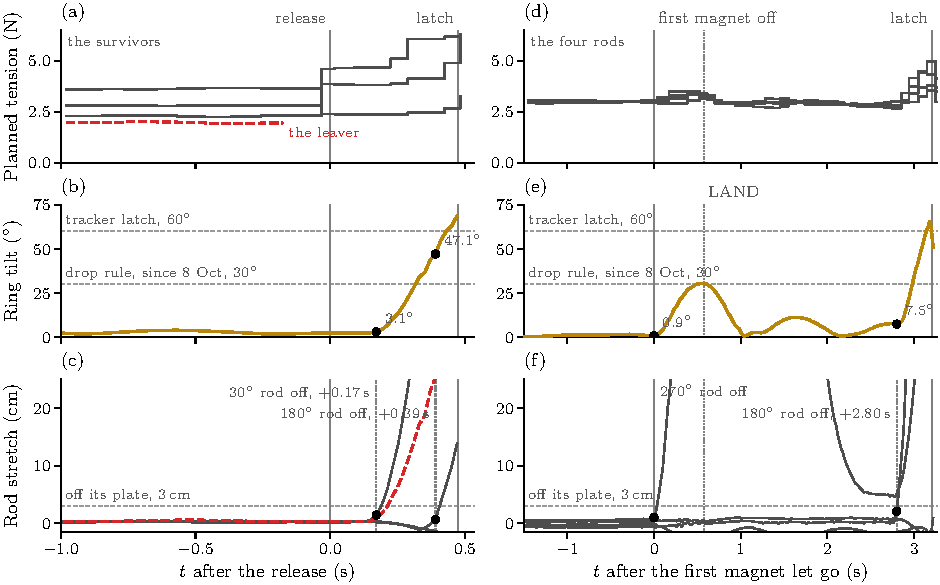
\includegraphics[width=\textwidth]{Images/magnet_anatomy.pdf}
\caption[How the ring was lost]{How the ring was lost on the rig, twice, both with the rods planned at 45$^\circ$.
Left, an announced release from the plate at 90$^\circ$ of a hover on the plates at 30, 90, 180 and 270$^\circ$ (a
150$^\circ$ gap left), on the planner's pull: (a) the planned tension per rod, the leaver's dashed, with the
survivors' step at the resize (2.8 to 4.6\,N and 2.3 to 3.8\,N on the two rods beside the gap); (b) the ring's tilt;
(c) each rod's measured length over its own, so that a rod leaving its plate shows as a rise: 0.17\,s after the
release the 30$^\circ$ rod let go with no command, at 2.6$^\circ$ of tilt, and the 180$^\circ$ rod followed at
0.39\,s; the trackers latched the fleet at 60$^\circ$ of tilt 0.47\,s after the release. Right, the circle at
0.125\,m/s on the measured pull with four rods on the even ring: (d) the planned tensions, 3.0\,N each; (e) the tilt;
(f) the 270$^\circ$ rod let go with no command at 0.9$^\circ$ of tilt and the ring recovered from 31$^\circ$; the
operator's LAND came 0.6\,s after it, and during the descent the 180$^\circ$ rod let go, at 7.7$^\circ$, and the ring
capsized. Dotted: the 30$^\circ$ drop rule and the trackers' 60$^\circ$ latch; the freed rods leave the panel.}
\label{fig:F11}
\end{figure}

% 12 Oct: the figure from branch thesis-figs (docs/figures/F_releases/caption.md) replaces the placeholder.
\begin{figure}[htbp]
\centering
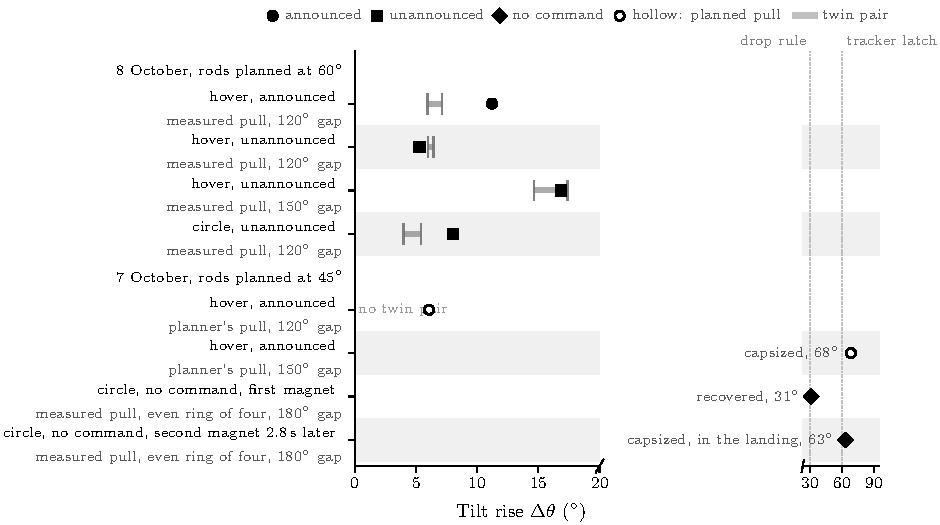
\includegraphics[width=\textwidth]{Images/releases.pdf}
\caption[Every release on the rig]{Every release on the rig, one row per event, grouped by the day and the rod
plan: the ring's tilt rise $\Delta\theta$ (the departure of its tilt vector from its mean over the 5\,s before the
event, over the event to LAND or to the fleet's latch) as a marker, filled for the measured rod pull and hollow for
the planner's pull, shaped by how the release came (announced, unannounced, or a magnet letting go with no command);
the grey bar with end ticks is the range of the twin pair flown on the same configuration, cut at the rig flight's
hold, and rows without one say so. The two capsizes and the one recovery sit on the broken axis against the
30$^\circ$ drop rule, which these flights predate, and the trackers' 60$^\circ$ latch. The 7 October circle flew the
even ring of four, whose three survivors leave a 180$^\circ$ gap; it lost two magnets 2.8\,s apart, recovered from the
first, and capsized on the second during the landing, so that row's pre-window holds the first recovery.}
\label{fig:F10}
\end{figure}

\paragraph{Where the survivors learn of the change.} [The frozen sign, then the outcome under the resolution rule.]

\pendingfig{fig:F12}{The other levers: (a) one-variable pairs (ramp on each pull source, resize timing, integral mode,
model error); (b) $\Delta\theta$ against the support margin, by pull source, with the rig points. [Caption.]}{Tier B
in the twin and the rig releases; L2 off-scale, marked as a magnet slip.}

\paragraph{What knowing about the release buys.} [Detection on against off, on both pull sources; scored on time back
in band, landing lean and clearance.]

\begin{table}[htbp]
  \centering
  \footnotesize
  \caption{The switch itself (T10), at the first live solve after a leave and after a join. [To fill.]}
  \label{tab:T10}
  \begin{tabularx}{\textwidth}{YYYYYY}
    \toprule
    Switch & Solver status & KKT residual & Gap to offline SQP & Solve time (ms, rig) & Throttle step (\%) \\
    \midrule
    Leave, announced & [\dots] & [\dots] & [\dots] & [\dots] & [\dots] \\
    Leave, unannounced & [\dots] & [\dots] & [\dots] & [\dots] & [\dots] \\
    Join (hand-over) & [\dots] & [\dots] & [\dots] & [\dots] & [\dots] \\
    \bottomrule
  \end{tabularx}
\end{table}

\paragraph{Answer to RQ2.} [Half a page.]
